\chapter{Wprowadzenie do tematyki pracy}
\label{cha:tematykaPracy}
Cyfrowa akwizycja obrazu pozwala na odwzorowanie widzialnej dla człowieka sceny w przestrzeni zdigitalizowanej. Takie przedstawienie obrazu umożliwia utrwalenie go na rozmaitych nośnikach pamięci i dostęp do niego w dowolnym momencie w przyszłości. Rejestrując zdjęcia z pewną częstotliwością i zachowaniem kolejności ich akwizycji otrzymuje się nagranie wideo. Pozwala ono śledzić zmiany na scenie następujące w czasie, takie jak ruch czy \textcolor{red}{zmiana} oświetlenia. Następujące po sobie obrazy zwane \textbf{ramkami} to \textbf{sekwencja wideo}.
\section{Preprocessing}
Choć dla człowieka informacje zawarte na obrazie są proste w interpretacji, maszyna ''widzi'' ramkę jako zwykły ciąg liczb. Dlatego aby dokonywać automatycznej detekcji pewnych zjawisk i zależności, należy poddać ją odpowiednim przekształceniom, pozwalającym wyekstrahować interesujące powiązania. Taki proces nazywa się przetwarzaniem wstępnym, czyli \textit{preprocessingiem}. W zależności od tego, jakie elementy ramki są w programie istotne, stosuje się różne metody uwydatnienia informacji. W książce \cite{i1823330731} opisane są najczęściej wykorzystywane algorytmy używane w takim procesie. W tej sekcji zostaną przedstawione niektóre z nich, istotne w kontekście niniejszej pracy.
\subsection{Binaryzacja}
Jest to jedna z podstawowych metod punktowego przetwarzania obrazu.  Pozwala odseparować istotne informacje na zdjęciu z pominięciem zależności mniej interesujących, takich jak na przykład konkretny poziom jasności, utrudniających tylko dalsze przetwarzanie ze względu na większą złożoność obliczeń. Obraz zostaje sprowadzony do postaci binarnej (zero-jedynkowej), gdzie najczęściej (w zależności od podejścia) 0 reprezentuje tło, 1 - interesujący obszar obrazu. \\
Istnieje wiele metod binaryzacji, dlatego też można wybrać odpowiednią dla każdego algorytmu. Podstawowym problemem staje się jednak wyznaczenie odpowiedniego progu binaryzacji - ze względu na następującą w procesie radykalną redukcję informacji zawartych w obrazie, źle dobrany graniczny poziom jasności może doprowadzić do błędnej detekcji, w konsekwencji skutkującej złym działaniem programu. Dlatego też bardzo ważna jest znajomość rodzaju danych, z jakimi system przetwarzający będzie miał do czynienia - pozwoli to zastosować odpowiednią dla nich metodę obliczenia progu.
\subsection{Przestrzenie barw}
Przestrzeń barw to pewna matematyczna reprezentacja światła widzialnego w przestrzeni cyfrowej. W zależności od potrzeb stosowane są różne modele. Najpopularniejszymi są spotykane w urządzeniach elektronicznych trójkanałowe RGB (ang. \textit{Red Green Blue}) oraz komplementarny do niego, stosowany w druku CMYK (ang. \textit{Cyan Magenta Yellow blacK}), wykorzystujące właściwości ludzkiego wzroku determinujące sposób, w jaki człowiek odbiera barwy. Każdemu pikselowi obrazu są tu przypisane odpowiednie wartości na każdym kanale, na przykład czerwony piksel w reprezentacji RGB na kanale czerwonym (R) ma maksymalną wartość 255 (w 8-bitowej głębi kolorów), na niebieskim i zielonym po 0. Stosowane są one do łatwej do interpretacji przez człowieka reprezentacji cyfrowej kolorów na zdjęciach. Wprowadzają one jednak duże ograniczenia ze względu na ilość niesionej informacji. Akwizycja obrazu w innej przestrzeni pozwala na przykład na zastosowanie o wiele szerszego spektrum barw. Dlatego też często przy przetwarzaniu obrazów stosuje się inne modele, rozdzielające istotne dla maszyny informacje na oddzielne kanały, co umożliwia wydajniejsze i niekiedy dokładniejsze obliczenia na zdjęciach. \\
W metodzie opisanej w rozdziale \ref{sec:BinWang}  używana jest przestrzeń YCbCr, oddzielająca kanał luminancji (Y), czyli poziomu jasności piksela, od kanałów chrominancji (Cb i Cr), przechowujących informację o jego odcieniu i nasyceniu. Taki sposób reprezentacji powstał z wykorzystaniem faktu, iż oko ludzkie jest o wiele bardziej czułe na poziom jasności obiektu, niż na jego kolor. Konwersja z przestrzeni RGB do YCbCr jest stosunkowo prosta - można ją zapisać w postaci macierzy:

\[
\begin{bmatrix}
    Y & Cb & Cr \\
\end{bmatrix}
=
\begin{bmatrix}
    R & G & B \\
\end{bmatrix}
\begin{bmatrix}
    0.299 & -0.168935 & 0.499813 \\
    0.587 & -0.331665 & -0.418531 \\
    0.114 & 0.50059 & -0.081282 
\end{bmatrix}
\]

Ponieważ wartości na kanałach RGB mieszczą się w przedziale 0-255, po przekształceniu do przestrzeni YCbCr otrzymujemy odpowiednio wartości od \[ 0-255\] na kanale Y oraz od \[-128-127 \] na kanałach Cb i Cr.
\begin{figure}[!htb]
\centering
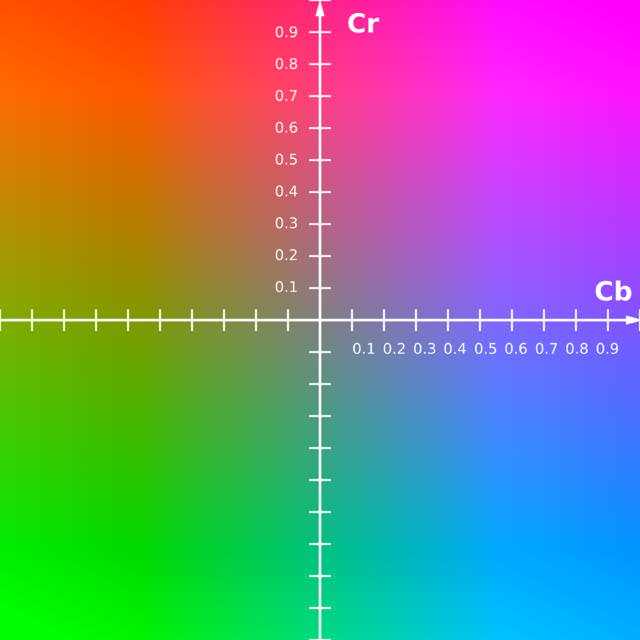
\includegraphics[width=82px]{img/YCbCr}
\caption{Reprezentacja płaszczyzny 
CbCr dla stałej luminancji Y=0.5}
%\floatfoot{Source: Wikipedia}
\end{figure}
\section{Analiza obrazu} 
\subsection{Segmentacja obiektów}
Po przekształceniach obrazu, uwydatniających zawarte w nim informacje, konieczne jest wyodrębnienie istotnych aspektów ramki. Służy do tego metoda zwana segmentacją obrazu, polegająca na podziale obrazu na segmenty odpowiadające konkretnym utrwalonym na nim elementom.
\section{Detekcja ruchu na scenie}
Detekcja ruchu, czyli \textit{Motion Detection}, to sposób wykrywania przemieszczania się obiektów na scenie względem ich sąsiedztwa. Polega ona na analizie kolejnych ramek z sekwencji wideo i badaniu zmian następujących pomiędzy nimi.\\
W wykrywaniu zmian pomagają algorytmy generacji tła.
\section{Standardowe metody generacji tła}
\subsection{Średnia bieżąca}
\cite{collins2003mean}
\subsection{Gaussian Mixture Model}
\label{sec:GMM}
Metoda ta \cite{zivkovic2004improved} opiera się na obserwacji, iż obiekty tła, przy braku przemieszczających się obiektów na scenie, wykazują pewne zależności, które mogą zostać przedstawione za pomocą modeli statystycznych. Dlatego też wyodrębnienie pikseli nie pasujących do takiego modelu wiąże się z wykryciem ruchu na scenie. Jest to stosunkowo mało skomplikowany algorytm oparty na mechanizmie subtrakcji tła.
\subsection{ViBE}
\cite{barnich2011vibe}
\subsection{PBAS}
\cite{hofmann2012background}
\section{Standardowe metody a dynamiczne tło}
\section{Narzędzia}
\subsection{Język C++}
\subsection{Biblioteka OpenCV}
\begin{figure}[!htb]
\centering


\includegraphics[width=82px]{img/ocv_logo}
\caption{Logo biblioteki OpenCV \cite{OpenCVLogo}}
%\floatfoot{Source: }
\end{figure}
OpenCV (ang. \textit{Open Source Computer Vision}) to dostępna od 2000 roku biblioteka, zawierająca implementacje najczęściej wykorzystywanych algorytmów wizyjnych. Jej główne zalety to dostępność na zasadach \textit{open source}, a także wieloplatformowość.\\
Została ona napisana w języku C, jednak istnieją specjalne nakładki, pozwalające korzystać z niej także m. in. w C++, C\#, Python i języku Java. Udostępniony publicznie jest nie tylko kod źródłowy, ale także i narzędzia, pozwalające na samodzielną kompilację biblioteki, co pozwala na używanie jej w wielu środowiskach programistycznych.
